\chapter{Projekt systemu}

\section{Ogólna architektura systemu}

System został zaprojektowany w celu nauki agenta, który skutecznie przechodzi poziomy w grze Super Mario Bros, wykorzystując algorytm Double Q-Learning. Architektura systemu składa się z czterech głównych komponentów: emulatora NES, agenta, algorytmu trenującego (DQN) oraz mechanizmu agregacji danych.

\subsection{Emulator NES}

Środowisko gry zostało zaimplementowane przy użyciu emulatora NES opartego na bibliotece \texttt{cynes} \cite{CYNES}. Emulator dostarcza informacje o stanie gry poprzez odczyt pamięci RAM oraz renderowanie obrazu gry w czasie rzeczywistym.

\subsection{Agent}

Agent w systemie to model decyzyjny, który podejmuje akcje w środowisku gry na podstawie bieżącego stanu. Model ten jest trenowany za pomocą algorytmu Double Q-Learning. Agent:

\begin{itemize}
	\item \textbf{Wejście:} Otrzymuje przetworzony obraz, generowany przez emulator \texttt{cynes}.
	\item \textbf{Wyjście:} Generuje sześć wartości odpowiadających naciśniętym klawiszom:
	      \begin{itemize}
		      \item cztery kierunki ruchu (lewo, prawo, góra, dół),
		      \item dwa przyciski akcji (A i B).
	      \end{itemize}
	\item \textbf{Cel:} Nauka optymalnej strategii, która maksymalizuje sumę nagród za pomocą algorytmu Double Q-Learning.
\end{itemize}
\subsection{Agregacja danych}

Mechanizm agregacji danych zajmuje się odczytem istotnych informacji ze stanu pamięci emulatora, takich jak pozycja Mario, prędkość, aktualny poziom, liczba punktów, a także stan przeciwników. Dane te są później używane do trenowania agenta. Tabela~\ref{tab:nes_memory} przedstawia najważniejsze zmienne i ich adresy w pamięci RAM.

\begin{table}[ht]
	\centering
	\caption{Zmienne odczytywane z pamięci emulatora NES}
	\label{tab:nes_memory}
	\begin{tabular}{|c|c|p{5cm}|}
		\hline
		\textbf{Adres w RAM}      & \textbf{Nazwa zmiennej}          & \textbf{Opis}                                         \\ \hline
		\texttt{0x75A}            & \texttt{lives}                   & Liczba żyć Mario.                                     \\ \hline
		\texttt{0x006D}           & \texttt{x\_horizontal}           & Pozioma pozycja Mario (wysoki bajt).                  \\ \hline
		\texttt{0x0086}           & \texttt{x\_on\_screen}           & Pozioma pozycja Mario na ekranie (niski bajt).        \\ \hline
		\texttt{0x0057}           & \texttt{horizontal\_speed}       & Prędkość pozioma Mario (w postaci liczby ze znakiem). \\ \hline
		\texttt{0x00CE}           & \texttt{y\_position\_on\_screen} & Pionowa pozycja Mario na ekranie.                     \\ \hline
		\texttt{0x0760}           & \texttt{level}                   & Aktualny numer poziomu gry.                           \\ \hline
		\texttt{0x07DD do 0x07E2} & \texttt{score\_bcd}              & Wynik punktowy w formacie BCD (Binary-Coded Decimal). \\ \hline
	\end{tabular}
\end{table}
\subsection{Przepływ danych w systemie}

\begin{figure}
	\begin{center}
		\begin{tikzpicture}[node distance=1.0cm]
			\node[draw, rectangle, minimum width=4cm, minimum height=0.7cm] (input) {Wejście: [60x64]};
			\node[draw, rectangle, minimum width=4cm, minimum height=0.7cm, below of=input] (conv1) {Warstwa konwolucyjna: 1 $\rightarrow$ 32};
			\node[draw, rectangle, minimum width=4cm, minimum height=0.7cm, below of=conv1] (bn1) {Warstwa normalizująca: 64 kanały};
			\node[draw, rectangle, minimum width=4cm, minimum height=0.7cm, below of=bn1] (conv2) {Warstwa konwolucyjna: 32 $\rightarrow$ 64};
			\node[draw, rectangle, minimum width=4cm, minimum height=0.7cm, below of=conv2] (bn2) {Warstwa normalizująca: 64 kanały};
			\node[draw, rectangle, minimum width=4cm, minimum height=0.7cm, below of=bn2] (flatten) {Spłaszczenie: 1x30720};
			\node[draw, rectangle, minimum width=4cm, minimum height=0.7cm, below of=flatten] (fc1) {Warstwa gęsta: 30720 $\rightarrow$ 128};
			\node[draw, rectangle, minimum width=4cm, minimum height=0.7cm, below of=fc1] (fc2) {Warstwa gęsta: 128 $\rightarrow$ 6};
			\node[draw, rectangle, minimum width=4cm, minimum height=0.7cm, below of=fc2] (output) {Wyjście: 6 wartości};

			% Connections
			\draw[->] (input) -- (conv1);
			\draw[->] (conv1) -- (bn1);
			\draw[->] (bn1) -- (conv2);
			\draw[->] (conv2) -- (bn2);
			\draw[->] (bn2) -- (flatten);
			\draw[->] (flatten) -- (fc1);
			\draw[->] (fc1) -- (fc2);
			\draw[->] (fc2) -- (output);

		\end{tikzpicture}
	\end{center}
\end{figure}

\begin{itemize}
	\item Agent odczytuje aktualny stan gry z pamięci emulatora, w tym pozycję Mario, liczbę żyć, prędkość i wynik.
	\item Na podstawie obrazu gry i odczytanych danych agent wybiera akcję za pomocą strategii \(\epsilon\)-greedy.
	\item Akcja jest przekazywana do emulatora w formie naciśniętych klawiszy.
	\item Emulator aktualizuje stan gry i zwraca wynikowe dane, które są zapisywane przez mechanizm agregacji.
\end{itemize}
\begin{figure}[ht]
	\begin{center}
		\resizebox{\textwidth}{!}{
			\begin{tikzpicture}[
					node distance=2.5cm, % Odstęp między węzłami
					align=center, % Wyśrodkowanie tekstu w węzłach
					>=latex, % Strzałki w stylu LaTeX
					%every node/.style={draw, text width=3cm} % Styl węzłów
				]

				\node[rectangle, minimum width=5cm, draw=black] (full_frame) {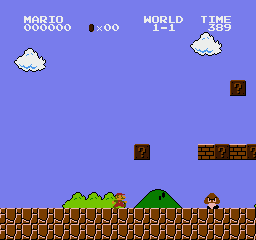
\includegraphics[width=4cm]{img/full_frame.png}\\Obraz generowany przez emulator NES};

				\node[right of=full_frame, xshift=6cm, draw=black] (compressed_frame) {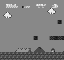
\includegraphics[width=2.5cm]{img/compressed_frame.png} \\Skompresowany obraz};
				\node (model) [right of=compressed_frame, draw = black, minimum height=2cm, xshift=2cm] {Model};

				\node (controller) [right of=model, draw=black, minimum height = 2cm, xshift=1cm, minimum width = 2cm] {Przyciski\\kontrolera\\NES};

				\draw[<-] (compressed_frame.west) -- (full_frame.east) node[midway] {Zmniejszenie\\ rozmiaru i \\ konwersja na skalę \\szarości};
				\draw[<-] (model.west) -- (compressed_frame.east) node[midway]{Konwersja\\na tensor};
				\draw[<-] (controller.west) -- (model.east) node[midway] {Predykcja\\wciśnięć};

			\end{tikzpicture}
		}
	\end{center}
	\caption{Ogólny schemat działania programu}
	\label{fig:sys_diagram}
\end{figure}
